\section{Innledning}
Eksperter i Team er et tverrfaglig emne som er obligatorisk for alle sivilingeniør- og mastergradsstudenter ved NTNU. Faget ble opprettet etter ønske fra næringslivet og har derfor et gjennomgående, yrkesforbredende fokus. Formål er å øke studentenes samarbeidskompetanse gjennom anvendelse av sin fagkunnskap i en gruppe med personer som har en annen, utfyllende kompetanse. Slik lærer studentene kommunikasjon- og samarbeids teknikker som skal bidra til helhetlige løsninger, trivsel og læring i et tverrfaglig prosjektarbeid og senere i arbeidslivet.

Formålet med prosessrapporten er å beskrive og reflektere rundt viktige hendelser med utgangspunkt i våre erfaringer, samarbeidsrelasjoner og dialoger underveis i prosessen. Noen av disse erfaringene har ført til spesifikke aksjoner, direkte knyttet til utviklingen av samarbeidet. Rapporten beskriver hendelser som har vært sentrale for denne utviklingen og som har vært viktige for fremgang og økt effektivitet i arbeidet med prosjektet.

\subsection{Gruppemedlemmene} %Her må det, natulig nok, bli et mer muntlig språk enn i resten av rapporten.
Personalia.

Faglig bakgrunn.

Forventninger til EiT.

Hvem er jeg? Hva studerer jeg? Hvordan ser jeg på min egen evne til samarbeid FØR EiT(gjerne noe negativt sånn at vi kan vise fremgang)? Hvilke forventninger har jeg til EiT?

\subsubsection{Karoline}
\begin{wrapfigure}{r}{0.5\textwidth}
  \vspace{-20pt}
  \begin{hfill}
    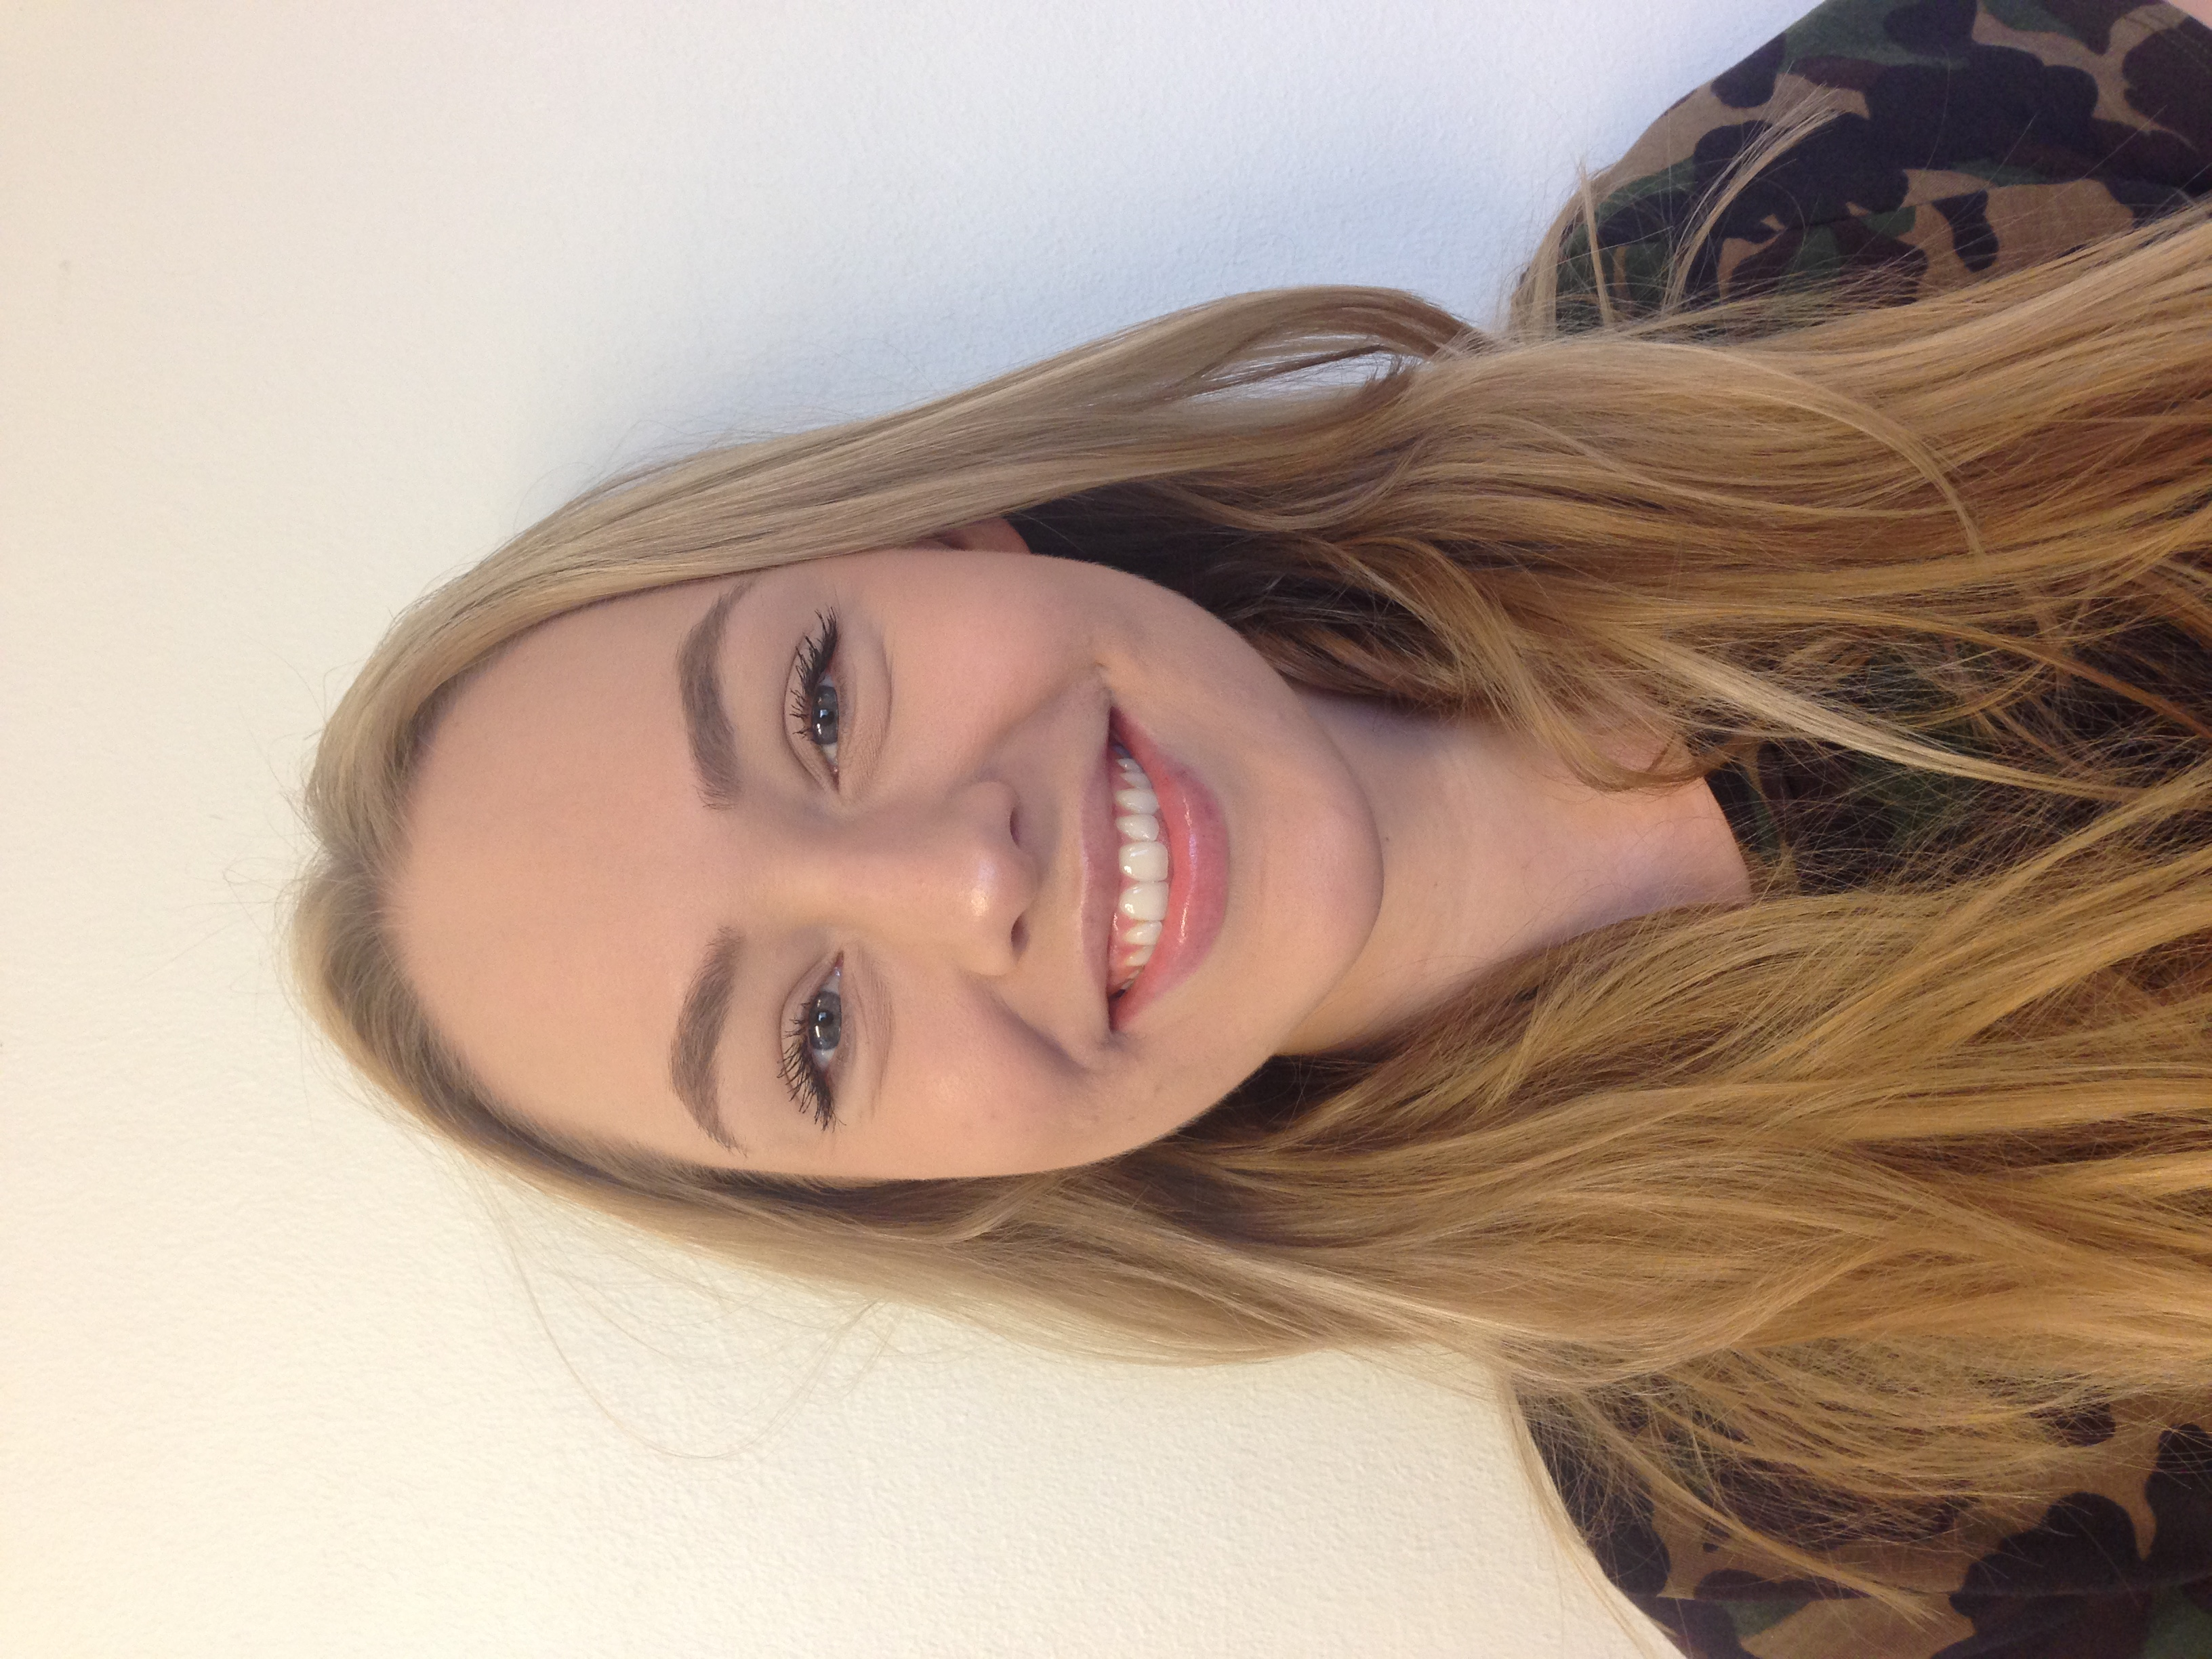
\includegraphics[scale=0.05, angle = 270, width=0.48\textwidth]{img_karoline.JPG}
  \end{hfill}
  \vspace{-12pt}
  %\caption{Ole Vebjørn Bakken}
  %\vspace{-10pt}
\end{wrapfigure}
Navnet mitt er Karoline Kroken, 22 år fra Sarpsborg og studerer en 5-årig master i Bygg og Miljøteknikk ved NTNU med fordypning innen bygg- og anleggsteknikk. De første årene i studieløpet bestod hverdagen min for det meste av selvstendig arbeid, men i løpet av det siste året har studieformen hovedsaklig vært preget av gruppeoppgaver og samarbeid. Av dette har jeg lært at selvom effektiviteten kanskje svekkes i et gruppearbeid, ser jeg stor verdi i å jobbe prosjektbasert sammen med andre som tenker ulikt meg selv. Av EiT forventer jeg å få tilbakemeldinger om hvordan jeg selv fungerer i en gruppesammenheng og hvordan jeg kan gjøre meg selv til den beste mulige samarbeidspartneren.Jeg har aldri jobbet på en tverrfaglig måte slik vi gjør i EiT, og jeg forventer utfordringer ved at alle ønsker "å dra i sin retning" i en gruppe bestående av studenter ved fire ulike studieprogram. Jeg ser på meg selv som en positiv og glad jente som kommer godt overens med andre mennesker. Jeg ser på mine evner til samarbeid som relativt gode, ved at jeg som person føler jeg verken tar for lite eller for mye plass. Dette kan også være min ulempe, vet at jeg ved noen anledninger kan mangle ansvarsfølelse eller tilhørighet til arbeidet. Jeg har også tidligere hatt tendenser til å kun engasjere meg i det jeg synes er spennende, og kan da lett falle ut av helheten i arbeidet. Jeg ser på EiT med stor seriøsitet fordi jeg vet at mitt yrkesliv i fremtiden vil bestå av prosjektarbeid med samarbeid på tvers av fag.

\subsubsection{Ole Vebjørn}
\begin{wrapfigure}{r}{0.5\textwidth}
  \vspace{-20pt}
  \begin{hfill}
    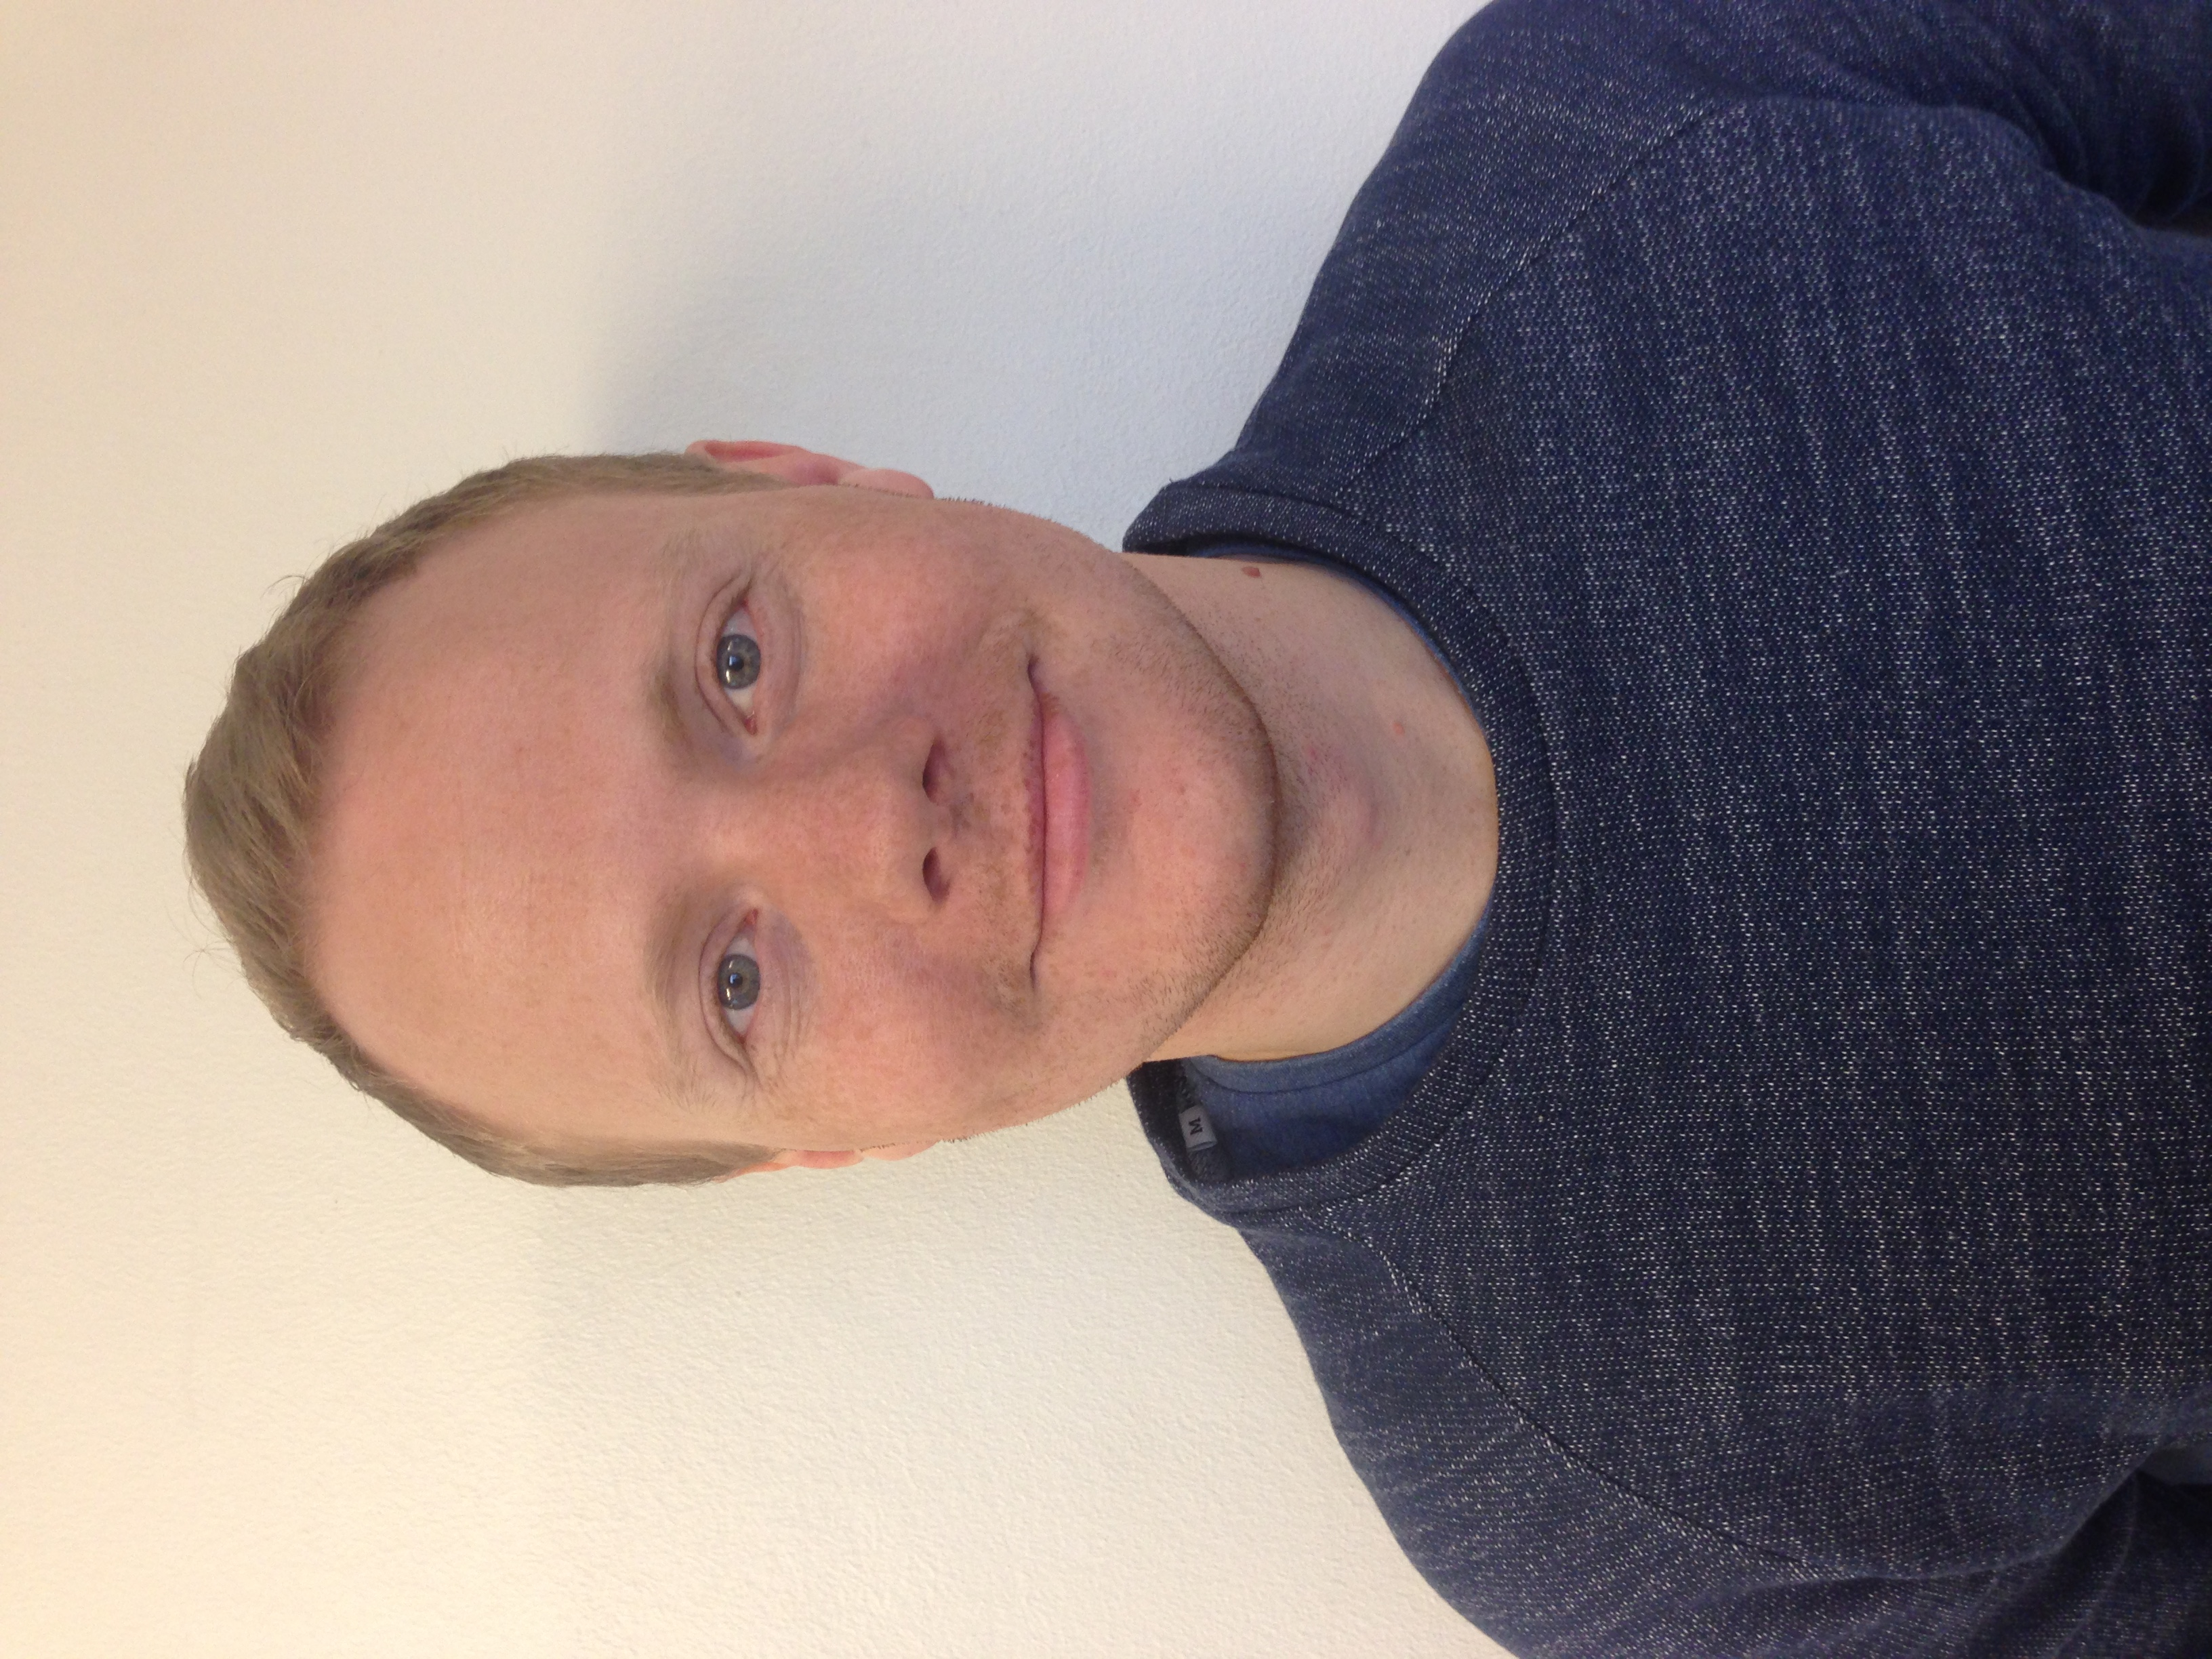
\includegraphics[scale=0.05, angle = 270, width=0.48\textwidth]{img_vebbe.JPG}
  \end{hfill}
  \vspace{-12pt}
  %\caption{Ole Vebjørn Bakken}
  %\vspace{-10pt}
\end{wrapfigure}
Jeg heter Ole Vebjørn Bakken, er 24 år og kommer fra Drammen. Jeg studerer en 2-årig master i Fysisk Planlegging ved NTNU og har fra tidligere en bachelor i Landskapsplanlegging med landskapsarkitektur ved Høgskulen i Sogn og Fjordane. Både min bachelorgrad- og mastergradutdanning er preget av mye prosjektarbeid i grupper. Jeg har gjennom studiene opparbeidet meg mye erfaring med å jobbe gruppe, noe jeg tar med meg inn i samarbeidet i EiT. Arbeid med arealplaner, steds- og landskapsanalyser, og kart- og visualiseringsprogrammer er faglige evner jeg også kan ta med meg inn i samarbeidet. I tidligere prosjektarbeid har jeg hatt ulike roller, noe som har gitt meg evner til å både være leder for gruppen og deltager. Jeg føler min egen evne til å samarbeide er meget god, der jeg kan både være tålmodig, rolig og engasjert. Min innstilling er at et gruppesamarbeid gir et bedre resultat enn et individuelt arbeid. Mine individuelle arbeidsferdigheter føler jeg er mindre gode, der jeg fort kan bli usikker på eget arbeid og ukonsentrert. Mine forventninger til EiT er å lære enda mer om å samarbeide i gruppe og bli bedre til å kjenne min egen rolle og egenskaper i et samarbeid. Siden tverrfaglige prosjektarbeid er en viktig del av mitt fagfelt og kommer mest sannsynlig til å være en stor del av min framtidige jobb, er jeg meget motivert for å ta til meg kunnskap og erfaring faget EiT vil gi.

\subsubsection{Iselin}
\begin{wrapfigure}{r}{0.5\textwidth}
  \vspace{-20pt}
  \begin{center}
    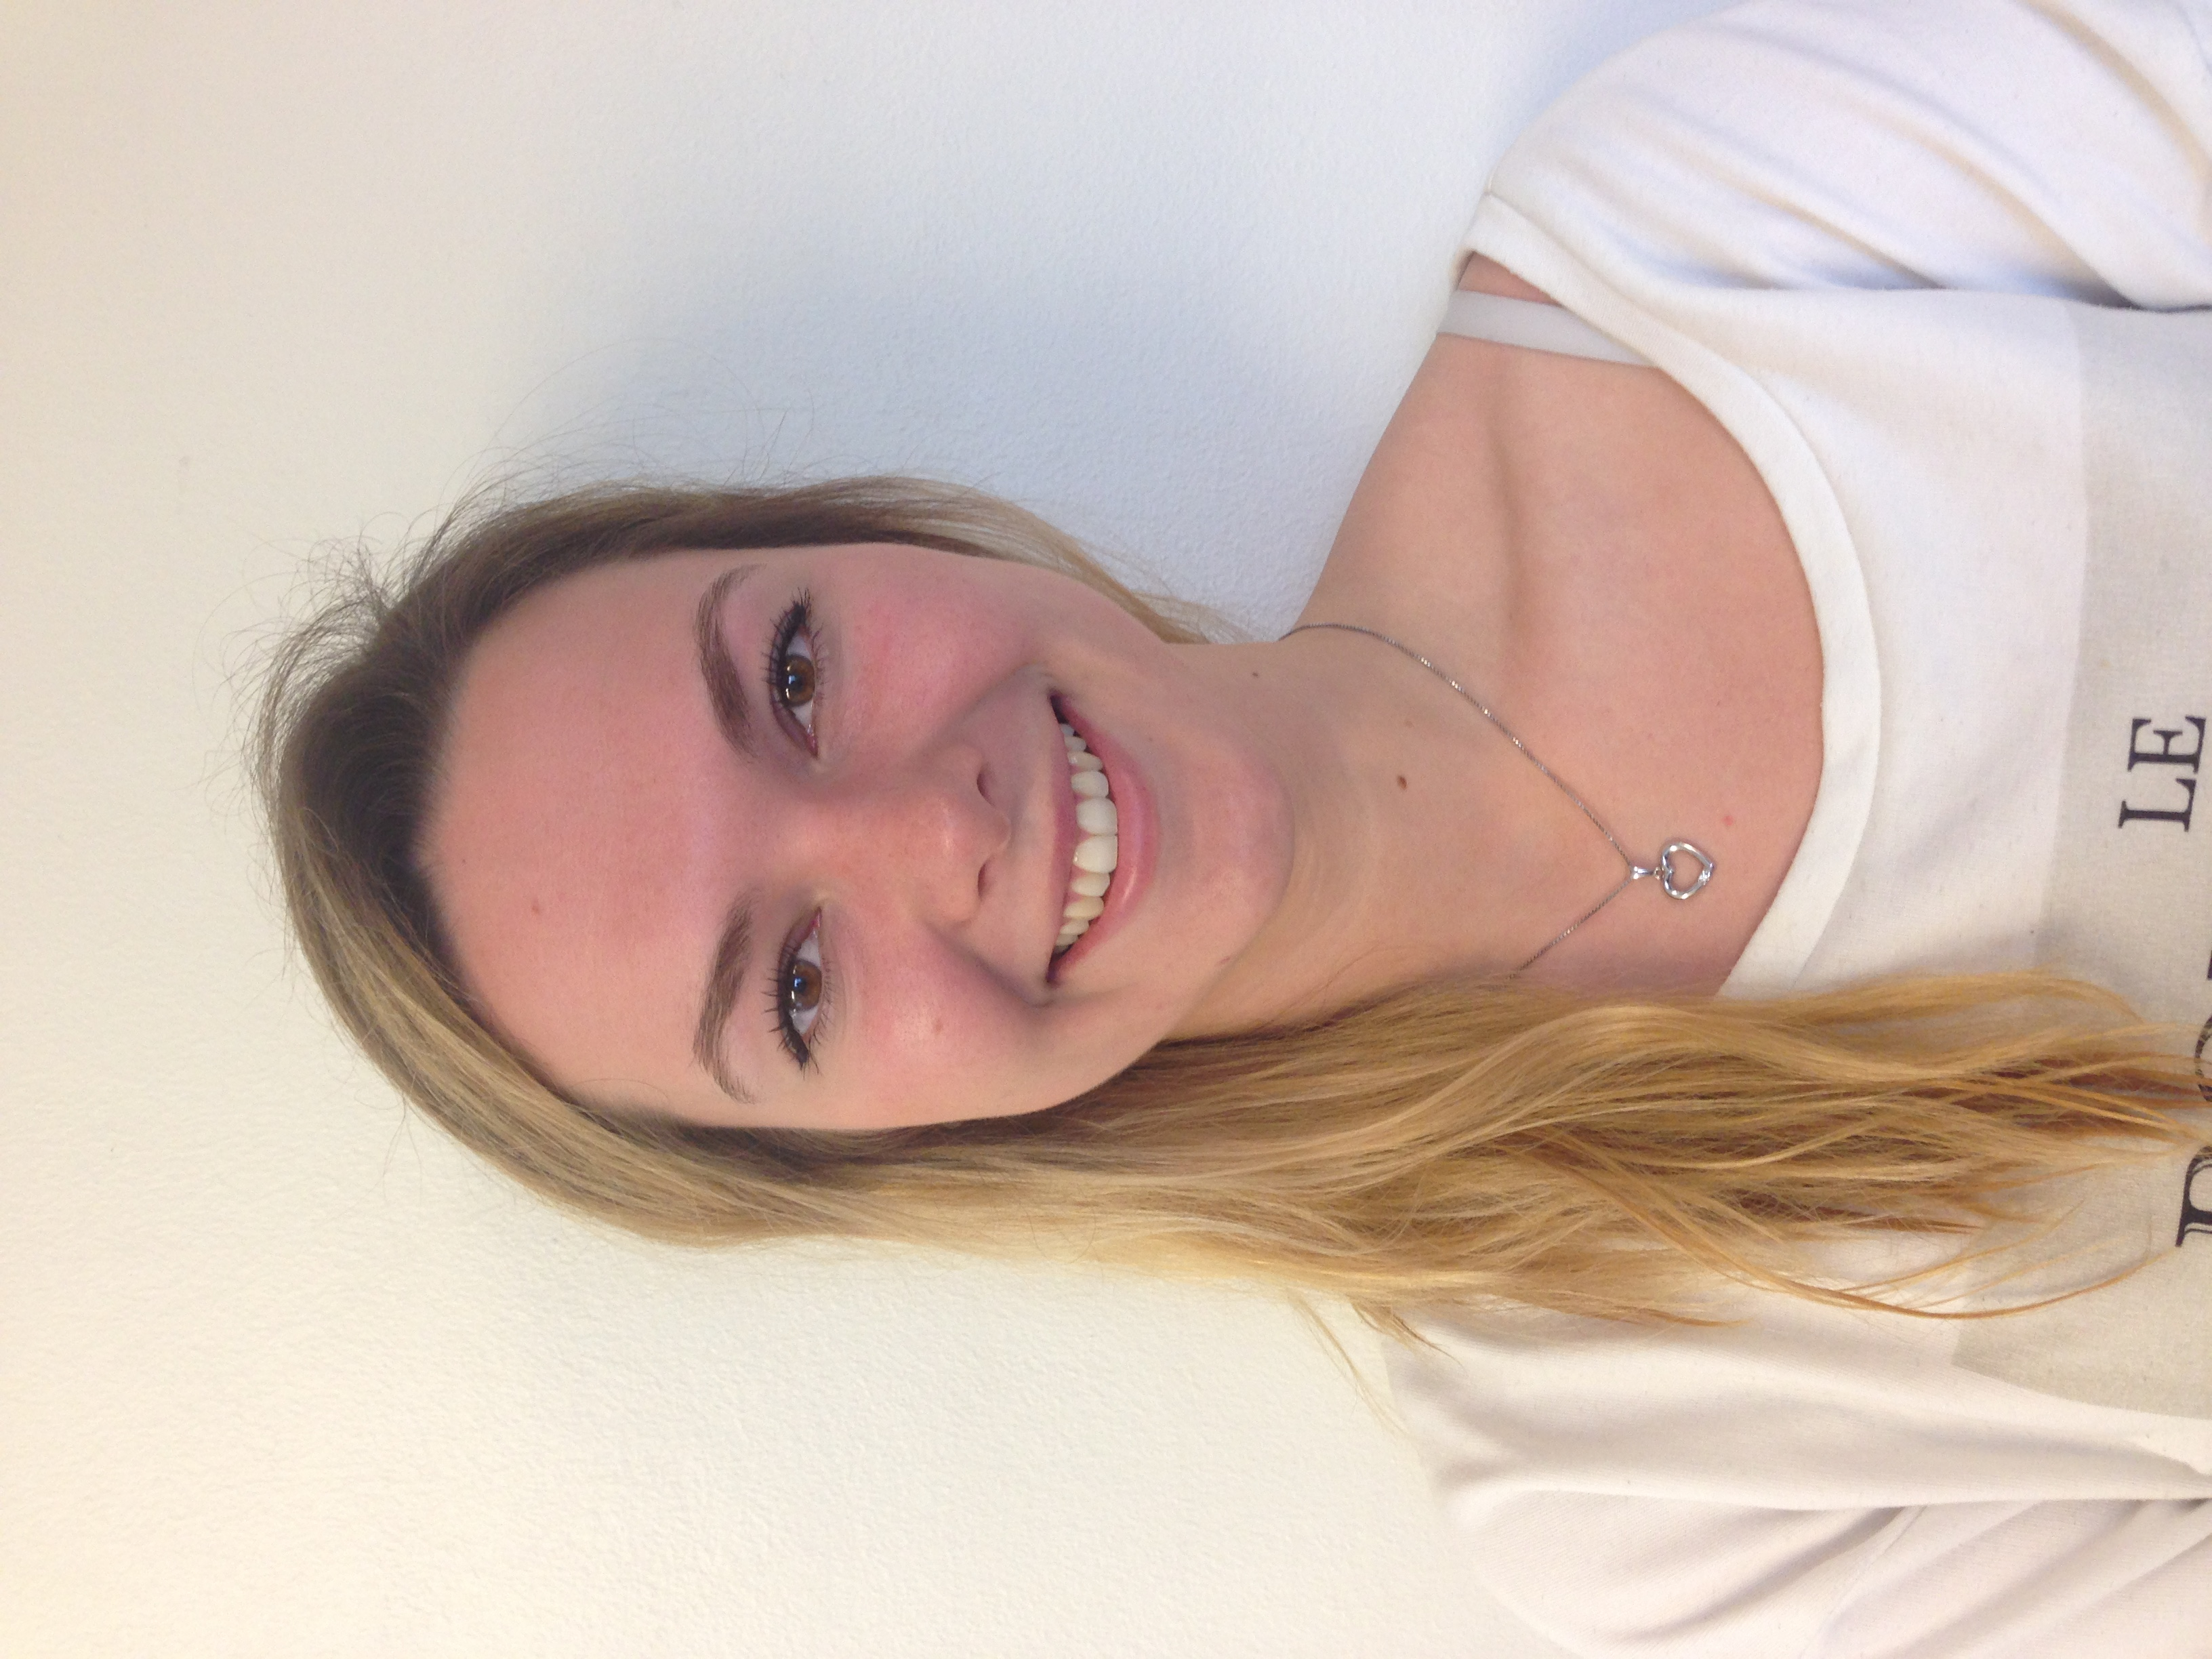
\includegraphics[scale= 0.02, angle = 270, width=0.48\textwidth]{img_iselin.JPG}
  \end{center}
  \vspace{-20pt}
  %\caption{Iselin Kanstad}
  \vspace{-10pt}
\end{wrapfigure}
Jeg heter Iselin Kanstad, er 24 år fra Asker, og jeg studerer en 5-årig master i Industriell Design med spesialisering innen interaksjonsdesign. I dette faget kan jeg bidra med designkompetanse, da særlig brukerforståelse, designmetodikk og grafiske fremstillinger, i tillegg til kreativitet og engasjement. Gruppearbeid er noe jeg er veldig vandt til fra studiet, da det å samarbeide er en av de viktigste kompetansene en designer kan ha. På studiet har vi som regel alltid minst to gruppebaserte fag, og jeg har også erfaringer fra tverrfaglige samarbeid fra noen fag og flere frivillige verv. Den første fordelen med gruppearbeid er etter min mening at beslutningene som taes blir preget av mange forskjellige synspunkt og at beslutningene derfor blir mer overveide. Det jeg ser som det største hinderet er at gruppearbeid ofte kan bli preget av dårlig effektivitet, derfor ser jeg også flere fordeler ved å jobbe selvstendig med enkelte oppgaver. Forventningene til faget er midt på treet, mye preget av å ha hørt om både positive og negative erfaringer fra andre studenter. Jeg håper å lære mye mer om gruppedynamikk og metodikk som kan taes i bruk for bedre samarbeid i en gruppe. 

\subsubsection{Mads}
\begin{wrapfigure}{r}{0.5\textwidth}
  \vspace{-20pt}
  \begin{center}
    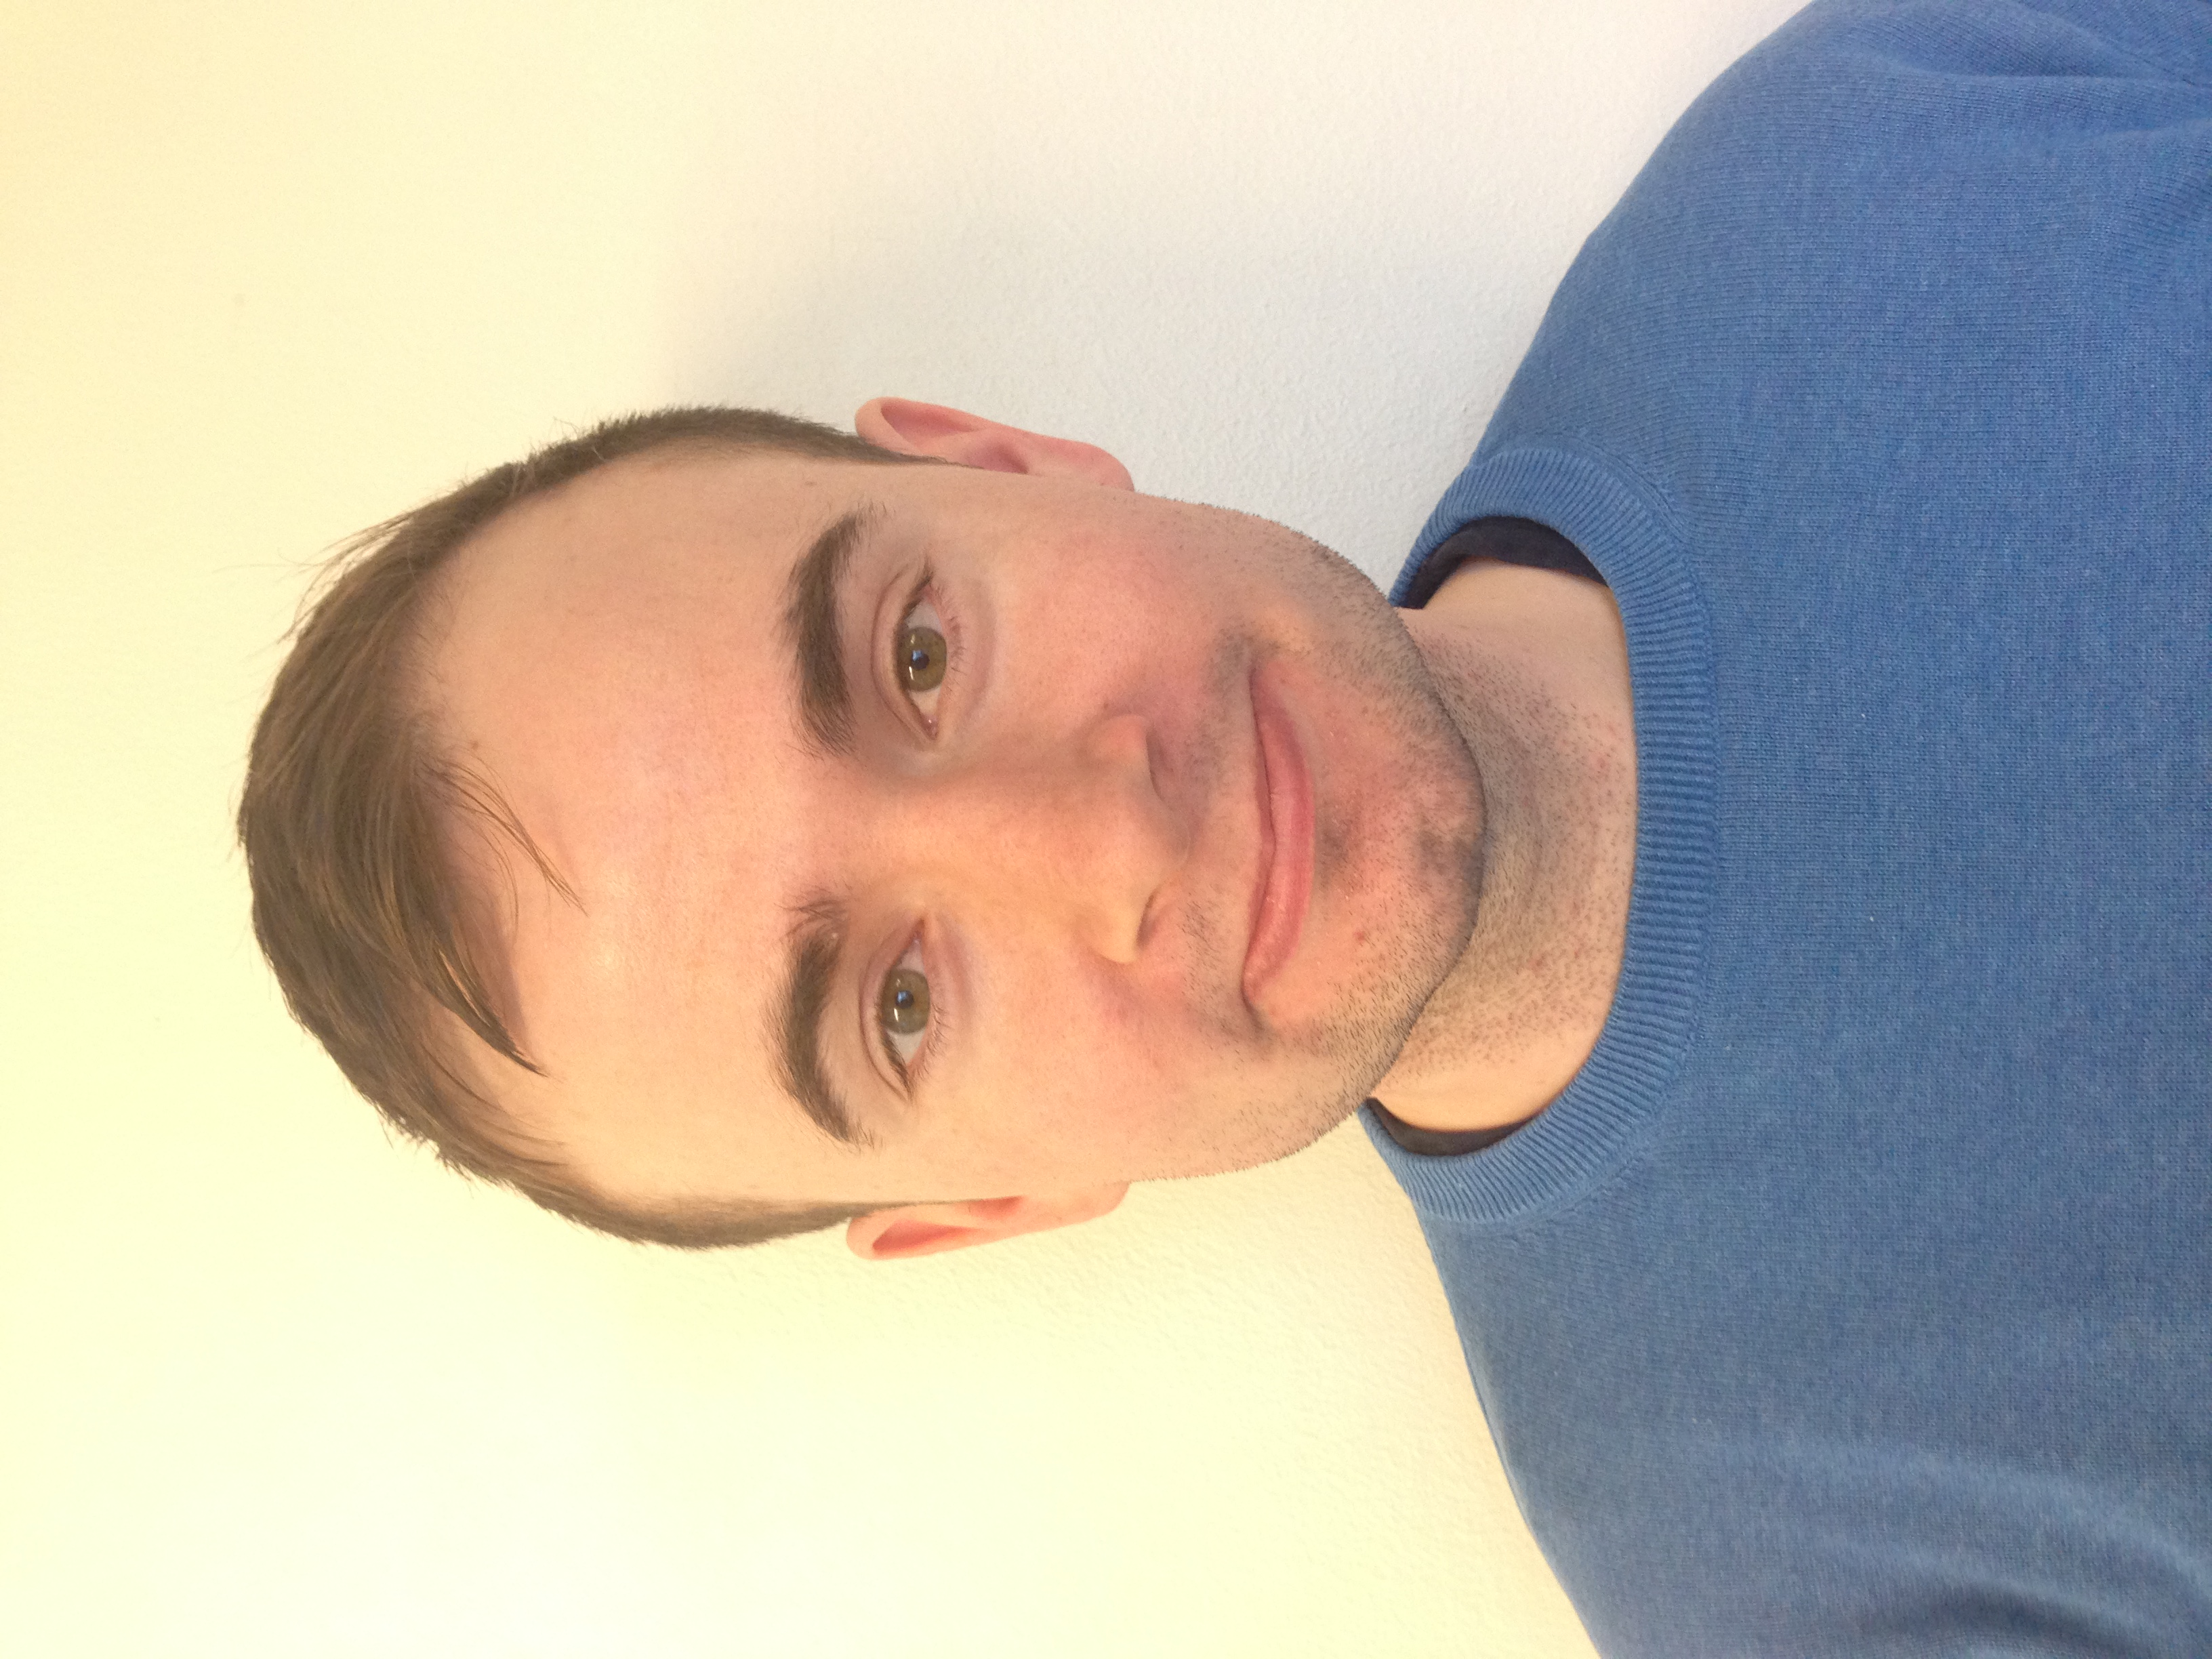
\includegraphics[scale= 0.02, angle = 270, width=0.48\textwidth]{img_mads.JPG}
  \end{center}
  \vspace{-20pt}
  %\caption{Mads Johan Laastad}
  \vspace{-10pt}
\end{wrapfigure}
Mitt navn er Mads Johan Laastad, er 25 år fra Bergen, og jeg studerer en 5-årig master i Teknisk Kybernetikk ved NTNU med en fordypning i biomedisinsk bevegelse. Det er en svært teknisk bakgrunn med hovedtyngde innen matematikk, programmering og reguleringsteknikk. Min vanlige studiehverdag er preget av mye selvstendig arbeid, og jeg liker best å jobbe med faglig arbeid alene. Fra militæret og frivillige verv har jeg fått erfare å ha lederansvar. I en ukjent gruppe mennesker vil jeg naturlig ta en lederrolle hvis ingen andre tar ansvaret. Det er også naturlig at jeg tar mye plass i en gruppe, og at jeg kan oppleves som intens av andre. Engasjert, løsningsorientert og pliktoppfyllende er beskrivende ord. Ved siden av studiene er jeg engasjert i studentdemokratiet og er ikke redd for å uttrykke mine meninger. Dette engasjementet har skapt mye dårlige forventninger til EiT gjennom skrekkhistorier fra studenter med dårlige opplevelser av faget. Mine forventninger til faget er derfor svært minimale. Mitt eneste håp er at jeg ikke havner på en gruppe med dårlig motiverte medstudenter som ikke føler tilhørighet til faget, har mye fravær eller mangler vilje til å gjøre en innsats. 

\subsection{Gruppefrafall}
Det var opprinnelig tiltenkt at elektronikk studenten Mattis Spieler Asp skulle være en del av denne EiT gruppen. De første to landsbydagene var det uklart hvorfor han ikke var tilstede. Etter den andre landsbydagen fikk Mads kontakt med Mattis på telefon. Han var i Frankrike på ferie og hadde ingen intensjon om å delta i EiT da han hadde søkt om fritak. Innen den fjerde landsbydagen ble det avklart at søknaden hadde gått gjennom, og at gruppen bare ville bestå av fire medlemmer.

Det er beklagelig at gruppen går glipp av de ressursene som Mattis kunne bidra med. Heldigvis gikk det ikke utover gruppesamholdet i den kritiske startfasen da han aldri var tilstede under landsbydagene og at situasjonen ble avklart innen rimelig tid. 

\subsection{Samarbeidsavtalen}
Gruppens samarbeidsavtale\footnote{Se vedlegg 5.3} ble produsert med referanse i et veiledningskriv vi fikk overlevert av landsbyleder. Her ble det skissert tre viktige momenter for en god samarbeidsavtale; leveranse, trivsel og læring. Dette danner grunnlaget for en modell som heter teamtrekanten\footnote{Hjertø (2008) etter Hackman(1987)}. Den viser hvordan leveranse, trivsel og læring er gjensidig avhengige av hverandre for å oppnå et godt teamarbeid.
\subsubsection{Leveranse}
Leveranse tar for seg hvordan vi evaluerer kvaliteten på det som leveres. Lengre var det en diskusjon på om utgangspunkt for selvevalueringen skulle være etter en normal karaktersetting. Gruppen gikk bort i fra dette da det var store forskjeller på hva den opplevde arbeidsinnsatsen må være for å oppnå en ønsket karakter. Spesielt var det Mads som hadde en helt annen oppfatning enn resten av gruppen over hva som måtte til for å oppnå en toppkarakter. Ordlyden i avtalen vektlegger istedenfor et individuelt ansvar om å bidra etter beste evne. 

Gruppen består kun av fire medlemmer, dette åpner for muligheten til å eksperimentere med en horisontal lederstrukturen. Ingen av medlemmene har tidligere erfaring med denne typen ledelse, og det ble ytret litt skepsis fra Mads. Han ønsket en mer tradisjonell leder og er bekymret over tapet av effektivitet en slik struktur vil medføre. Argumentet for denne strukturen er at det bidrar til økt kreativitet og en mer balansert maktdynamikk i gruppen \footnote{Kilde?}. Etter en diskusjon kommer gruppen frem til at det kunne være interessant å forsøke med horisontal lederstruktur og at beslutningen skal revurderes sammen med samarbeidsavtalen.

Det defineres også hvilke kommunikasjons plattformer gruppen skal bruke. Det skilles mellom en ren faglig plattform og en informasjonsflyt/planleggings plattform. Arbeidstiden defineres som en full arbeidsdag hver onsdag frem mot innlevering, med mulighet for helgearbeid ved behov. Behandling av fravær blir også utdypet i denne delen av avtalen.

\subsubsection{Trivsel}
Dette delen av avtalen skal ta for seg hvordan det skal sikre et godt arbeidsmiljø og trivsel blant gruppemedlemmene for å fremme et godt samarbeid.

Dette er et viktig tema for gruppen. Alle er enige om at et godt arbeidsmiljø er avgjørende for et godt samarbeid. 

Det etableres en "konflikt-timeout" som det kraftigste verktøyet for å bli hørt av resten av gruppen. Alle medlemmene kan til enhver tid be om en "timeout". Dette prioriteres over alt annet arbeid, og må umiddelbart behandles av hele gruppen. Formålet med dette er å skape en trygg formidlingsplattform for medlemmene. Her kan alle ta opp det de ønsker med resten av gruppen, og normalt arbeid kan ikke gjenopprettes før personen som ba om en "timeout" er fornøyd med tiltakene. Alt skal loggføres og tiltakene skal revurderes fortløpende.

Krevende avgjørelser som ikke viser tegn til en løsning eller kompromiss etter lengre tid med diskusjoner kan bli avgjort gjennom avstemning. Formålet er å gi gruppen et verktøy for å avslutte ressurskrevende diskusjonsrunder som har stagnert eller ikke viser noen fremgang mot et kompromiss.

Det legges ned et rammeverk for felles pauser og lunsj. Da må alle forlate arbeidsplassen sammen og helst trekke litt frisk luft utendørs. Det er ikke tillatt med faglig diskusjon i løpet av pausen. Formålet var å skape et tydelig skille mellom arbeid og rekreasjon. Samtidig gir det medlemmene muligheten til å bli bedre kjent i en uformell setting.

\subsubsection{Læring}
Her skal det tilrettelegges for kompetanseheving og mestring av fremtidige samarbeids oppgaver blant gruppemedlemmene.

Tilbakemeldinger og fasilitering fra veilederne gir grunnlag for en umiddelbar "timeout". Her skal tilbakemeldingen analyseres grundig, og på grunnlag av denne analysen skal gruppen vurdere om det er nødvendig med tiltak. 

Ærlige og konkrete tilbakemeldinger internt i gruppen er viktig. For Karoline kan det være en utfordring å motta direkte tilbakemeldinger, men  det er generell enighet om å fremme disse verdiene fremfor å være vage i frykt for å støte enkelte medlemmer. Derfor blir det også vedtatt at alle tilbakemeldinger skal formidles på en ordentlig måte, være konstruktive og ha en god intensjon om et bedre samarbeid som bakgrunn. Læringsutbyttet vil også være svært avhengig av at alle kan være trygge på tilbakemeldingene er så profesjonelle som mulig og ikke personlig. 

Knyttet til dette blir det også vedtatt at alle må ta imot tilbakemeldingene uten å gå i forsvarsposisjon. Mads formidler ovenfor resten av gruppen at dette er noe han må jobbe med fremover. 

\subsection{Revurdert samarbeids avtale} 
%Her drøftes det, så kanksje seksjonen burde flyttes til hoveddel/avslutning?
Det ble gjort noen små endringer fra den originale samarbeids avtalen. Hovedsakelig var dette kun mindre presiseringer i teksten med ett unntak; det ble fjernet referanser til et eksternt dokument som skulle utdype kvaliteten på det utførte arbeidet. Etterhvert som vi arbeidet ble det tydelig at alle medlemmene var dedikert i arbeidet, og det ble ikke opplevd noen uoverensstemmelser mellom de individuelle arbeidsinnsatsene. Derfor var det aldri behov for en nærmere utdypelse av arbeidskvaliteten i samarbeidsavtalen. 

\subsubsection{Leveranse}
Det store diskusjons-momentet for denne delen av avtalen var hvorvidt gruppen skulle ha en horisontal lederstruktur. Her fikk Mads mye rett i sin prediksjon av tapt effektivitet og manglende fremdrift. Det var til tider i starten svært lite fremgang og lite effektivitet. Halvveis i semesteret ble det diskutert om vi skulle endre på strukturen. Tidspunktet dette ble diskutert er viktig, for gruppen stod da ovenfor en omfattende og viktig beslutning over hvilke retning arbeidet skulle ta. Det hadde vært flere omfattende diskusjonsrunder uten resultat og Mads ønsket da å ta diskusjonen om lederstrukturen. Han mente en tydelig definert leder skal være i stand til å ta slike vanskelige beslutninger hvis ikke gruppen kommer til enighet selv. Etter en diskusjonsrunde endret han derimot mening. Det ble sett på som et nederlag for samarbeidet og en billig løsning på problemet hvis den eneste måten å løse uenighetene på var å velge en leder. Dessuten ville gruppedynamikken endre seg drastisk i en så liten gruppe. Med bare fire medlemmer ville en leder være det avgjørende stemmen i en splittet avgjørelse, og diskusjonen ville endre karakter fra å overtale hele gruppen til å kun overtale lederen. Dette var ikke noe gruppen ønsket, og valget var derfor å beholde den horisontale lederstrukturen.

Kommunikasjons plattformene har vært effektive og fungert etter hensikt. Store mengder materiale er produsert og blitt lagret på en oversiktlig måte på nettplattformer hvor alle medlemmene har hatt tilgang.

\subsubsection{Trivsel}
Innføringen av "timeout" har vært en stor suksess. Til tider ble den brukt flere ganger hver landsbydag, men det har aldri blitt opplevd som misbrukt. Flere av de beste grupperefleksjonene har blitt skapt takket være denne formidlingsplattformen.

Bruk av avstemninger har derimot ikke vært så vellykket. Det har vært tilfeller hvor diskusjonen rundt bordet er fastlåst og alle klausuler for å avholde en avstemning har vært tilstede, likevel har det ikke blitt gjennomført etter hensikt. Dette ble forsøkt ved et par anledninger, men gruppen fikk ikke noe positivt ut av det og valgte heller videre diskusjon i håp om å komme til enighet. Derfor er det i praksis aldri blitt brukt avstemning for å avgjøre en splittet avgjørelse. Det har derimot blitt brukt avstemninger til et helt annet formål; å avgjøre om den gjeldende diskusjonen er oppfattet som unødvendig av flertallet i gruppen. Dette har flere ganger spart gruppen for unødvendige diskusjoner og gruppen ser på det som en nyttig implementasjon av ordningen.

\subsubsection{Læring}
Gruppen har pliktoppfyllende loggført alle tilbakemeldinger fra veilederne. Hver eneste gang har fasiliteringen sin relevans blitt evaluert av gruppen. Her har Mads vært den mest kritiske røsten og forklarer dette med at han alltid er svært kritisk til informasjonskilder. Resten av gruppen har ikke opplevd denne kritikken for useriøs, og det har ofte vært til stor hjelp under analysen av tilbakemeldingene.

Gruppen har vært svært gode på å gi ærlige tilbakemeldinger til hverandre. Karoline har virkelig jobbet godt med sin evne til å motta og formidle konstruktiv kritikk, og Mads har etter hvert blitt mye mer mottakelig for tilbakemeldinger fra gruppen. De gode fremskrittene skyldes mest sannsynlig et høyt fokus på å skape et trygt arbeidsmiljø hvor ønsket om å hjelpe hverandre bli bedre samarbeidspartnere står sterkt.

\subsection{Fravær}
Som beskrevet i samarbeidsavtalen så skal alle forsinkelser eller fravær varsles på forhånd. I tillegg ble fraværet loggført i et eget dokument slik at negative handlingsmønstre kunne bli avdekket så tidlig som mulig.

\begin{tabular}{l*{6}{c}r}
Fravær[minutter] & Iselin & Vebbe & Karoline & Mads & Kommentar\\
\hline
Dag 1 & 0 & 0 & 0 & 0 \\
Dag 2 & 0 & 0 & 0 & 0 \\
Dag 3 & 18 & 2 & 0 & 21 & Bussforsinkelse\\
Dag 4 & 0 & 0 & 0 & 0 \\
Dag 5 & 0 & 0 & 0 & 0 \\
Dag 6 & 6 & 0 & 1 & 0 \\
Dag 7 & 1 & 0 & 0 & 0 \\
Dag 8 & 7 & 0 & 0 & 0 \\
Dag 9 & 0 & 0 & 0 & 0 \\
Dag 10 & 0 & 0 & 0 & 0 \\
Dag 11 & 150 & 135 & --- & 0 & \parbox[t]{5cm}{Karoline var syk. Iselin og Ole-Vebjørn var hos legen.}\\
Dag 12 & 0 & 0 & 0 & 0 \\
Dag 13 & 0 & 0 & 0 & 0 \\
Dag 14 & 0 & 0 & 0 & 0 \\
Dag 15 & 0 & 0 & 0 & 0 \\
\hline
Totalt: & 0 & 0 & 0 & 0 \\
\end{tabular}

\subsection{Refleksjoner} %Prosess, metode, øvelse..
Gruppen har kommet frem til en metode for å dokumentere refleksjoner på slutten av hver landsbydag. Det er et selvutviklet verktøy som baserer seg på teknikker beskrevet i refleksjonshåndboken, men siden flere aspekter er egenprodusert ønsker gruppen å utdype fremgangsmåten nærmere.

Metoden skal hjelpe individuelle medlemmer og gruppen som helhet til å oppnå bedre samarbeid. Gruppen går gjennom den på slutten av hver landsbydag og det settes av litt over en time til gjennomføringen. I begynnelsen tok metoden mye tid og ressurser av gruppen, men det ble sett på som en investering i et bedre og mer effektivt samarbeid. Den består av fire trinn; individuell refleksjon, individuell tilbakemelding, situasjon-refleksjon-aksjon(SRA) og grupperefleksjon. Resultatene fra de tre siste trinnene ble loggført fra hver landsbydag i et fellesdokument.

\subsubsection{Individuell refleksjon}
Metoden starter med at medlemmene skriver ned private refleksjoner rundt individuel innsats og samarbeidet i gruppen. Privat refleksjon skal ikke deles med resten av gruppen. Formålet med denne øvelsen er å øke selvinnsikten og refleksjon rundt egenutviklingen blant medlemmene i gruppen.

\subsubsection{Individuelle tilbakemeldinger}
Neste steg i metoden er en gruppeøvelse. Medlemmene trekker frem et utvalg av positive og negative sider ved eget bidrag i løpet av landsbydagen. Erfaring viser at dette ofte er en konkretisering av den individuelle refleksjonen. Etter hvert innlegg får resten av gruppen mulighet til å kommentere. Her kan gruppen reflektere rundt momentene som medlemmene tar opp. Ofte har det vist seg av gruppen er uenig med individet sin egenoppfatning. For eksempel kan et medlem oppleve seg selv som passiv i diskusjonene, mens gruppens mening er at dette ikke er tilfelle. På denne måten forsterkes utbytte av den individuelle refeleksjonen i trinnet over.

\subsubsection{Situasjon-refleksjon-aksjon}
Hvis det har oppstått situasjoner i løpet av landsbydagen av en betydelig karakter skal det bli tatt opp på situasjon-refleksjon-aksjon(SRA) trinnet. Episoder, situasjoner eller holdninger som påvirker samarbeidet bli analysert av gruppen gjennom et fast handlingsmønster. Et godt kjennetegn på en slik situasjon er at den bryter med den fastlagte gruppedynamikken og skaper et klart definert avvik fra gruppen eller individets handlingsmønster. Dette er ikke et kriterium, men hvis det gjennomføres en timeout av en i gruppen så skal dette føres som en SRA situasjon. Øvelsen beskriver først situasjonen, så reflekterer gruppen rundt situasjonen og til slutt bestemmes aksjoner for å bevare eller endre situasjonsgrunnlaget. Øvelsen dokumenterer både ønsket og uønsket påvirkning av gruppen og danner et grunnlag for å øke gjenkjenning og aktiv endring eller bevaring av etablerte handlingsmønstre.

\subsubsection{Grupperefleksjon}
Siste trinnet i metoden er en grupperefleksjon på slutten av landsbydagen. Først vurderes forskjellige aksjonstiltak fra tidligere SRA gjennomganger. Det diskuteres om aksjonene har fungert etter hensikt og om det er behov for endringer. Til slutt skrives en kort generelt oppsummering av gruppesamarbeidet for den aktuelle landsbydagen. Dette hjelper gruppen til å løfte blikket og å danne seg en overordnet situasjonsoversikt.
